%===================================== CHAP 2 =================================

\chapter{Literature Review and Background}

%Web and experience, enric pliaza, ralph bergmann, CBR stuff cooking recepies

%Mining stories from web
\section{Related work}
Discuss other articles that touch on the same subject

\subsection{Text data mining} \label{sec_tdm}
This projects aims at extracting specific sections from articles on Wikipedia and then find relations among them. This puts this project in between two fields. On one side there is information retrieval(IR), which is mainly is about helping users finding documents of their needs\cite{irbook}. On the other side is text data mining(TDM), where the goal is to discover useful information from textual data. Methods for accomplishing this could for instance be finding patterns across data sets, or finding relevant information among a collection of mostly irrelevant data\cite{untanglingTDM}.

To be able to discover relevant data from the Wikipedia articles, Wikimedia's markup language has to be interpreted. Section \ref{wikimedia} explains further about Wikimedia and the syntax of its markup, this section will focus on the structure we can derive from the markup. This structure mainly consists of section headers and the content of an section below, although there is also other information that can be extracted. To find relation between articles we would also need to look at the semantics from this information, were the most important is lists, categories and references, amongst others. YAWN\footnote{Yet Another Wikipedia Annotation project}, is a project that created an XML version of Wikipedia with focus on semantic information\cite{yawn}. The XML corpus produced by YAWN is general for the whole Wikipedia and the entire articles. This project only focuses on the articles relevant for educational purposes and possessing examples to explain its content. Although YAWN overreaches our purpose, key concepts and techniques for exploiting the Wiki markup, can be derived and used for classifying examples in this project. The most interesting for this project is how they find semantic annotations for Wikipedia pages. For that, they use a combination of exploiting information from categories assigned to articles and deriving information from the structure of an article.

Our project will make heavy use of categories to discover relations between examples, but we believe there still exists other information in the articles to further increase the accuracy of the relations discovered. Internal links between articles is another way we can mine data about relations between articles. Links also forces us to consider the difference between a link going into an article, and a link going from one. Evgeniy Gabrilovich and Shaul Markovitch used Wikipedia as a knowledge repository in an effort to enhance text categorization\cite{text-cat}. They made use of links and their sometimes differing \textit{anchor texts} (Display text of the link) ti improve their text categorization. A concept they took advantage of were that different anchor texts for the same link can indicate different contexts.  They also looked at number of incoming links to an article. Our project aims to look at bit deeper into the links between articles. We hope to utilize the information gained by knowing that one article links to another and how that connects them. David Milne and Ian H. Witten looks more into this connection between articles in their approach,  Wikipedia Link-based Measure (WLM)\cite{wlm}. Here they used mainly to methods to measure the relatedness between two articles, based on links. The first one is an approach similar to the TF;IDF algorithm, where they count links instead of terms. They then create vectors according to the vector space model and then finds the similarity of two articles based on the angle of their vectors. The second method they use are modeled after the Normalized Google Distance\cite{gsd}. Here the simply assumes that two articles containing the same link indicates relatedness. On the other hand, if one article contain a specific link which the other do not, indicate the opposite.



\subsection{Wikimedia} \label{wikimedia}
Wikimedia\cite{wikimedia} is an organization that supports and operates many different knowledge projects. Their goal is to make free knowledge accessible anywhere and on any platform. Their income comes primarily from donations. They do not make us of ads, because they believe it could jeopardize their reliability as a neutral source of information.

The project Wikimedia is mostly known for, is Wikipedia\cite{wikipedia}. Wikipedia is the largest collection of free, collaborative knowledge that exists. Wikipedia has can be found in over 290 languages and across those, contains more than 35 million articles. This project will make use of the English Wikipedia, which contains more than 5 million articles. Wikipedia uses a  software called MediaWiki\cite{mediawiki}. It is a server side software used for hosting wiki sites. Many of the wiki sites under the Wikimedia umbrella makes use of MediaWiki. A part of the MediaWiki software is the markup language used for writing articles. This markup, written by contributors, will then later be translated into HTML when displayed for users in their web browser. This markup is used to create elements such as tables, equations, lists and links. Wikimedia regularly backs up Wikipedia and makes it publicly available by dumping it to a large XML file. This gives access to the raw data that makes an article, which is meta data in XML format and the content of the article using the syntax of the MediaWiki markup. 

Public access to this information gives a lot of opportunities. Alberto Montero-Asenjo and Carlos A. Iglesias used a XML dump from the Spanish Wikipedia for language research\cite{lr-wiki}. They created a piece of software that processes the raw source data from the XML dump. It starts by converting the Wiki markup into plain text and then use further operations on the plain text to make the end result of useful data. While they use the raw data for language research, this projects needs to extract more information from the source data beyond what is contained in a plain text version. This means that this project has to interpret the syntax and the semantics behind it, instead of filtering it away.
How to interpret the sematics which the markup reveals has been touched on and discussed in section \ref{sec_tdm} and a couple of articles\cite{text-cat}\cite{wlm}. There is though a surprisingly lack of work about the interpretation of the markups syntax itself. Because of this, we have had to build this from the ground up with help from a Wikipedia page created for assisting people creating the articles\footnote{\url{https://en.wikipedia.org/wiki/Help:Wiki_markup}}. You can read more about how this project solved this in section \ref{cap_3} and \ref{cap_4}.



\subsection{SMILA} \label{smila}

\begin{figure}[h]
\caption{An overall overview of the SMILA architecture}
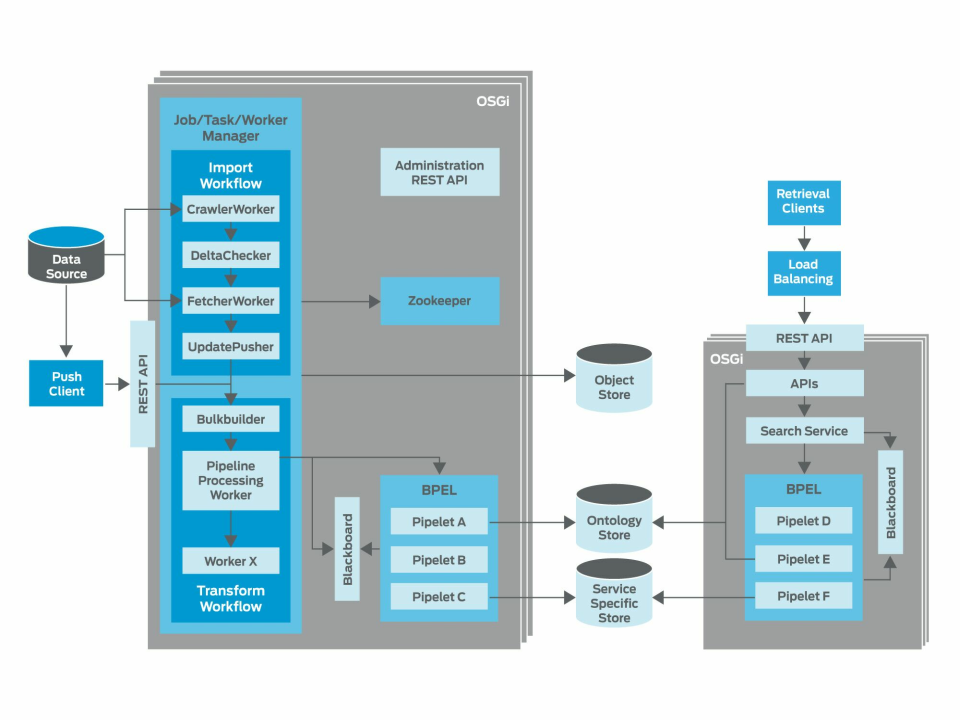
\includegraphics[width=\textwidth]{SMILA_Architecture}
\end{figure}

%%fix sånn abbrevation for SMILA

%%når jeg snakker om mine erfaringer med smila gjør jeg det i implementation.

%%Skriv om dette til å passe til sin nye kontekst
In the early stages of the project, an existing project called SMILA\cite{smila} was explored. SMILA is a system with its first release in 2010, is used to search and access unstructured information. SMILA crawls the web to extract information and then stores the information in an index. It has a REST API to control the system and for searching the index. The SMILA architecture is also based on the pipeline architecture containing the following processes; jobs, crawling, storage, indexing and querying. Since 2010, 6 new versions has been released adding more features to SMILA. With SMILA being very complex, it gains asynchronicity as its biggest benefit from the pipeline architecture. The SMILA pipeline also allows custom made pipelets to be inserted into the pipeline. A pipelet is a sub process inside a pipeline. By creating pipelets, the behaviour of SMILA could be tailored into extracting relevant information from Wikipedia.

The releases for SMILA has been dwindling the last three years with only 1 release in 2015. If you add that to the fact that all the different features of SMILA makes it very complex, the usability and stability suffers. This was experienced during testing of the program during this project.
Nevertheless the utility that the SMILA system offers could be taken advantage of in this project. Either by utilizing SMILA itself, or look at how SMILA retrieves data from the web, processes it and produces a data set as a result.


\section{Tools / Methodology}

\subsection{ElasticSearch} \label{elasticsearch}
%%JSON abbrevation
ElasticSearch is a tool used in this project for indexing the examples. ElasticSearch is built on top of Apache Lucene(https://lucene.apache.org), which is a information retrieval library, written in Java. Internally in ElasticSearch, data is stored as structured JSON\footnote{JSON - JavaScript Object Notation} documents. The API for communicating with ElasticSearch is a RESTful\footnote{REST - representational state transfer} API using JSON over HTTP. The API can be used for configuring ElasticSearch, building the index and querying it. 
%%Ta med i erfaring seksjon om dette at siden alt dette bruker json og webserveren bruker javascript via node, er alt veldig enkelt og konsistent.

ElasticSearch is built for scalability. This means that it can handle the dataset and interactions growing. This is because it acts as a cluster of many nodes. If the system needs to scale, new nodes can easily be added, and ElasticSearch will distribute resources to the newly added ndoes. However this projects does not need or take advantage of this scaling, and will only be using one node.

When searching in ElasticSearch, there is mainly two ways of doing this. The first one is by using \textit{filter}. The \textit{filter} is utilizing \textit{term} to decide whether a document should be returned or not. Searching with \textit{term} is very similar to how one would use SQL. %Trenger denne forklaring?
Searches can for instance consist of text strings, numbers, ranges or dates, and ElasticSearch will return everything that matches. It also allows for boolean operators and nesting of these. Using a \textit{filter} is very quick and should be used if the relevance of the documents is not important. If relevance score is important then the second option, \textit{query}, should be chosen. If a \textit{query} is combined with a \textit{term}, ElasticSearch is looking for the exact value in its index. A score is then returned based on the documents TF/IDF relevance to the term. See section \label{tfidf} for an explanation of this algorithm.%Burde det referes på denne måten?
If a \textit{match} is used instead, an analysis will be performed, creating a list of terms from the query, and then executing low-level queries for each of the terms. The results are combined to produce the final relevance score. These two methods can also be combined or extended with other methods to customize the search further.


\subsection{NPM and Node.js}
Two of the processes used by this project are written in JavaScript. JavaScript are normally run inside browsers, but by using Node.js\cite{node} the can be executed by a server. Node is an asynchronous event driven framework. By embracing to event loop in this manner, Node avoids thread management and blocking of those. Instead callbacks are pushed on too the event loop and Node runs until there are no more callbacks to perform.


\section{Techniques}

\subsection{Pipeline} \label{pipeline}
Describe a software pipeline. Advantages and stuff.\\
How should i use references for this?

\subsection{TF/IDF} \label{tf/idf}
TF/IDF is an algorithm which calculates how important an word is to a document based on the document itself and the collection it is part of. Based on this it is possible to decide how likely it is for the document to be relevant. TF/IDF is used as the standard similarity algorithm in ElasticSearch, see section \ref{elasticsearch}.

TF/IDF is can be divided into two parts, \textit{term frequency} and \textit{inverse document frequency}. \textit{Term frequency} is how often a term appears in a document. The more instances the document has of the word, the higher is the chance of the document being relevant. \texit{Inverse document frequency} looks at how often a term appears in the whole collection of documents. The more often a term appears, the less relevant is the term. This means the common terms will have less weight than rare ones, when calculating the likelihood of the documents relevance. 

\cleardoublepage